\documentclass{article}

\usepackage[colorlinks, urlcolor=blue, linkcolor=red, citecolor=green]{hyperref}
\usepackage{fancyhdr} %设置页眉和页脚的
\usepackage{extramarks} %设置continue那玩意的
\usepackage{amsmath}
\usepackage{amsthm}
\usepackage{amsfonts}
\usepackage{tikz} %画线的
\usepackage[plain]{algorithm}
\usepackage{algpseudocode}
\usepackage{enumerate}

\usetikzlibrary{automata,positioning}

%表
\usepackage{booktabs}
\usepackage{multirow}
\usepackage{array}
\usepackage{caption}
\DeclareCaptionFont{heiti}{\heiti} %还可以定义其他的
\captionsetup{labelsep=space, font={small, bf}, skip=2pt} %space可以改成quad

%图
%*****************图片及其相关设置***************************
\usepackage{graphicx}
\graphicspath{{tupian/}}
\usepackage{subfigure}

%*****************代码相关设置***************************
\usepackage{pythonhighlight}
%
% Basic Document Settings
%

\topmargin=-0.45in
\evensidemargin=0in
\oddsidemargin=0in
\textwidth=6.5in
\textheight=9.0in
\headsep=0.25in

\linespread{1.1}

\pagestyle{fancy}
\lhead{\hmwkAuthorName}
\chead{\hmwkClass: \hmwkTitle}
\rhead{\firstxmark}
\lfoot{\lastxmark}
\cfoot{\thepage}

\renewcommand\headrulewidth{0.4pt}
\renewcommand\footrulewidth{0.4pt}

\setlength\parindent{0pt}

%
% Create Problem Sections
%

\newcommand{\enterProblemHeader}[1]{
    \nobreak\extramarks{}{Problem \arabic{#1} continued on next page\ldots}\nobreak{}
    \nobreak\extramarks{Problem \arabic{#1} (continued)}{Problem \arabic{#1} continued on next page\ldots}\nobreak{}
}

\newcommand{\exitProblemHeader}[1]{
    \nobreak\extramarks{Problem \arabic{#1} (continued)}{Problem \arabic{#1} continued on next page\ldots}\nobreak{}
    \stepcounter{#1}
    \nobreak\extramarks{Problem \arabic{#1}}{}\nobreak{}
}

\setcounter{secnumdepth}{0}
\newcounter{partCounter}
\newcounter{homeworkProblemCounter}
\setcounter{homeworkProblemCounter}{1}
\nobreak\extramarks{Problem \arabic{homeworkProblemCounter}}{}\nobreak{}

\newenvironment{homeworkProblem}{
    \section{Problem \arabic{homeworkProblemCounter}}
    \setcounter{partCounter}{1}
    \enterProblemHeader{homeworkProblemCounter}
}{
    \exitProblemHeader{homeworkProblemCounter}
}

%
% Homework Details
%   - Title
%   - Due date
%   - Class
%   - Section/Time
%   - Instructor
%   - Author
%

\newcommand{\hmwkTitle}{Homework\ \#1}
\newcommand{\hmwkDueDate}{February 21, 2021}
\newcommand{\hmwkClass}{Machine Learning}
\newcommand{\hmwkClassTime}{}
\newcommand{\hmwkClassInstructor}{Professor Xiao Li}
\newcommand{\hmwkAuthorName}{Peng Deng}
\newcommand{\hmwkAuthorSchool}{School of Data Science}
\newcommand{\hmwkAuthorNumber}{Sno.220041042}
%
% Title Page
%

\title{
    \vspace{2in}
    \textmd{\textbf{\hmwkClass:\ \hmwkTitle}}\\
    \normalsize\vspace{0.1in}\small{Due\ on\ \hmwkDueDate}\\
    \vspace{0.1in}\large{\textit{\hmwkClassInstructor\ \hmwkClassTime}}
    \vspace{3in}
}

\author{\textbf{\hmwkAuthorName}}

\date{}

\renewcommand{\part}[1]{\textbf{\large Part \Alph{partCounter}}\stepcounter{partCounter}\\}

%
% Various Helper Commands
%

% Useful for algorithms
\newcommand{\alg}[1]{\textsc{\bfseries \footnotesize #1}}
\usepackage[algo2e,vlined,ruled]{algorithm2e}

% For derivatives
\newcommand{\deriv}[1]{\frac{\mathrm{d}}{\mathrm{d}x} (#1)}

% For partial derivatives
\newcommand{\pderiv}[2]{\frac{\partial}{\partial #1} (#2)}

% Integral dx
\newcommand{\dx}{\mathrm{d}x}

% Alias for the Solution section header
\newcommand{\solution}{\textbf{\large Solution}}

% Probability commands: Expectation, Variance, Covariance, Bias
\newcommand{\E}{\mathrm{E}}
\newcommand{\Var}{\mathrm{Var}}
\newcommand{\Cov}{\mathrm{Cov}}
\newcommand{\Bias}{\mathrm{Bias}}
\begin{document}

\maketitle
\thispagestyle{empty}

\newpage
\setcounter{page}{1}

\begin{homeworkProblem}
	[20 points] Suppose that $Y=\{0,1\}, P(Y=0)=P(Y=1)=\frac{1}{2}.$ $X$ is a continuous random variable with probability density function given by
	$$
		\begin{array}{l}
		p_{X \mid Y}(x \mid y=0)=\left\{\begin{array}{cc}
		e^{-x}, & x \geq 0 \\
		0, & \text { \textit{otherwise} }
		\end{array}\right. \\
		\\
		
		p_{X \mid Y}(x \mid y=1)=\left\{\begin{array}{lc}
		\frac{1}{2}, & x \in[a, a+2] \\
		0, & \text { \textit{otherwise} }
		\end{array}\right.
		\end{array}
	$$
	
	where $a \geq 0$
	\begin{itemize}
	    \item[(a)] Skecth $p_{X \mid Y}(x \mid y=0)$ and $p_{X \mid Y}(x \mid y=1)$
	    \item[(b)] If $X=\frac{1}{2},$ find the most likely value of $Y$ by using Bayes' Theorem. What about $X=1 ?$
	\end{itemize}
	
	\vspace{4pt}
	\textbf{\large{Solution}}
	
	\vspace{4pt}
	\textbf{Subproblem (a)}
	
	The plots of $p_{X \mid Y}(x \mid y=0)$ and $p_{X \mid Y}(x \mid y=1)$ are showed in Figure \ref{pdf}.
	\begin{figure}[H]
		\centering
		\subfigure[Probability density function 1]{\label{newton}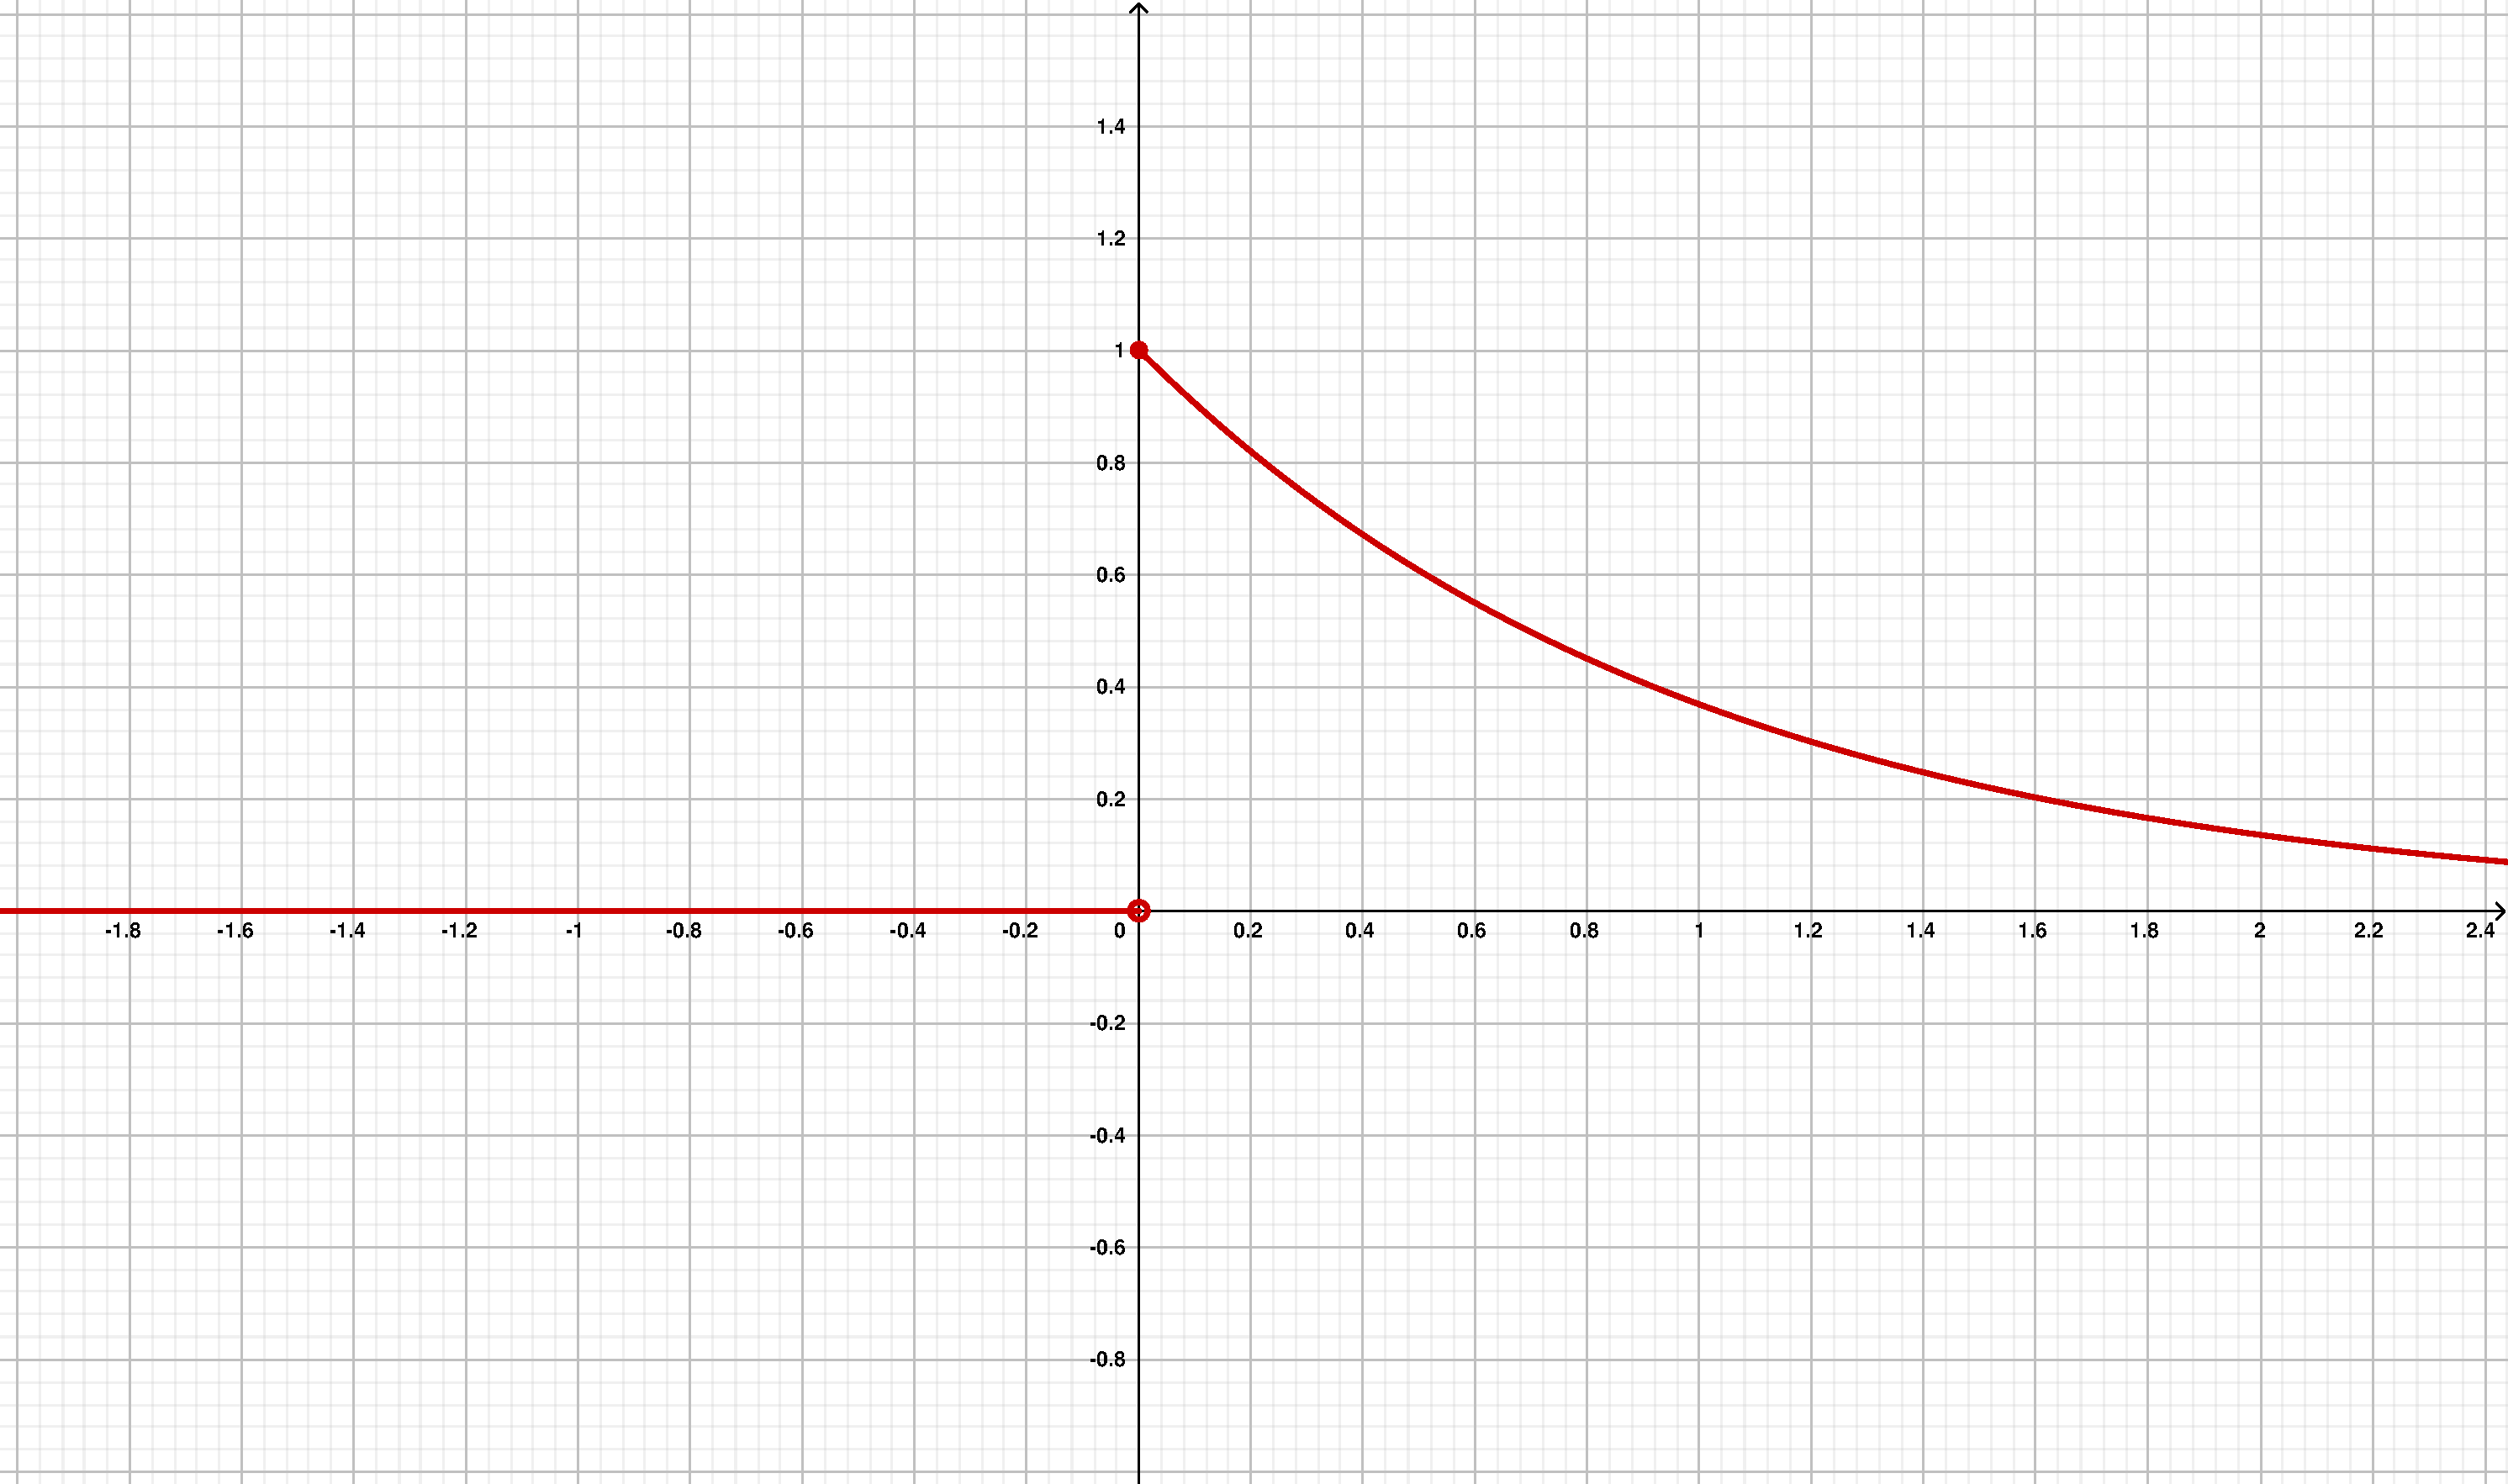
\includegraphics[width=0.6\linewidth]{pdf1}}
		\quad
		\subfigure[Probability density function 2]{\label{convergence}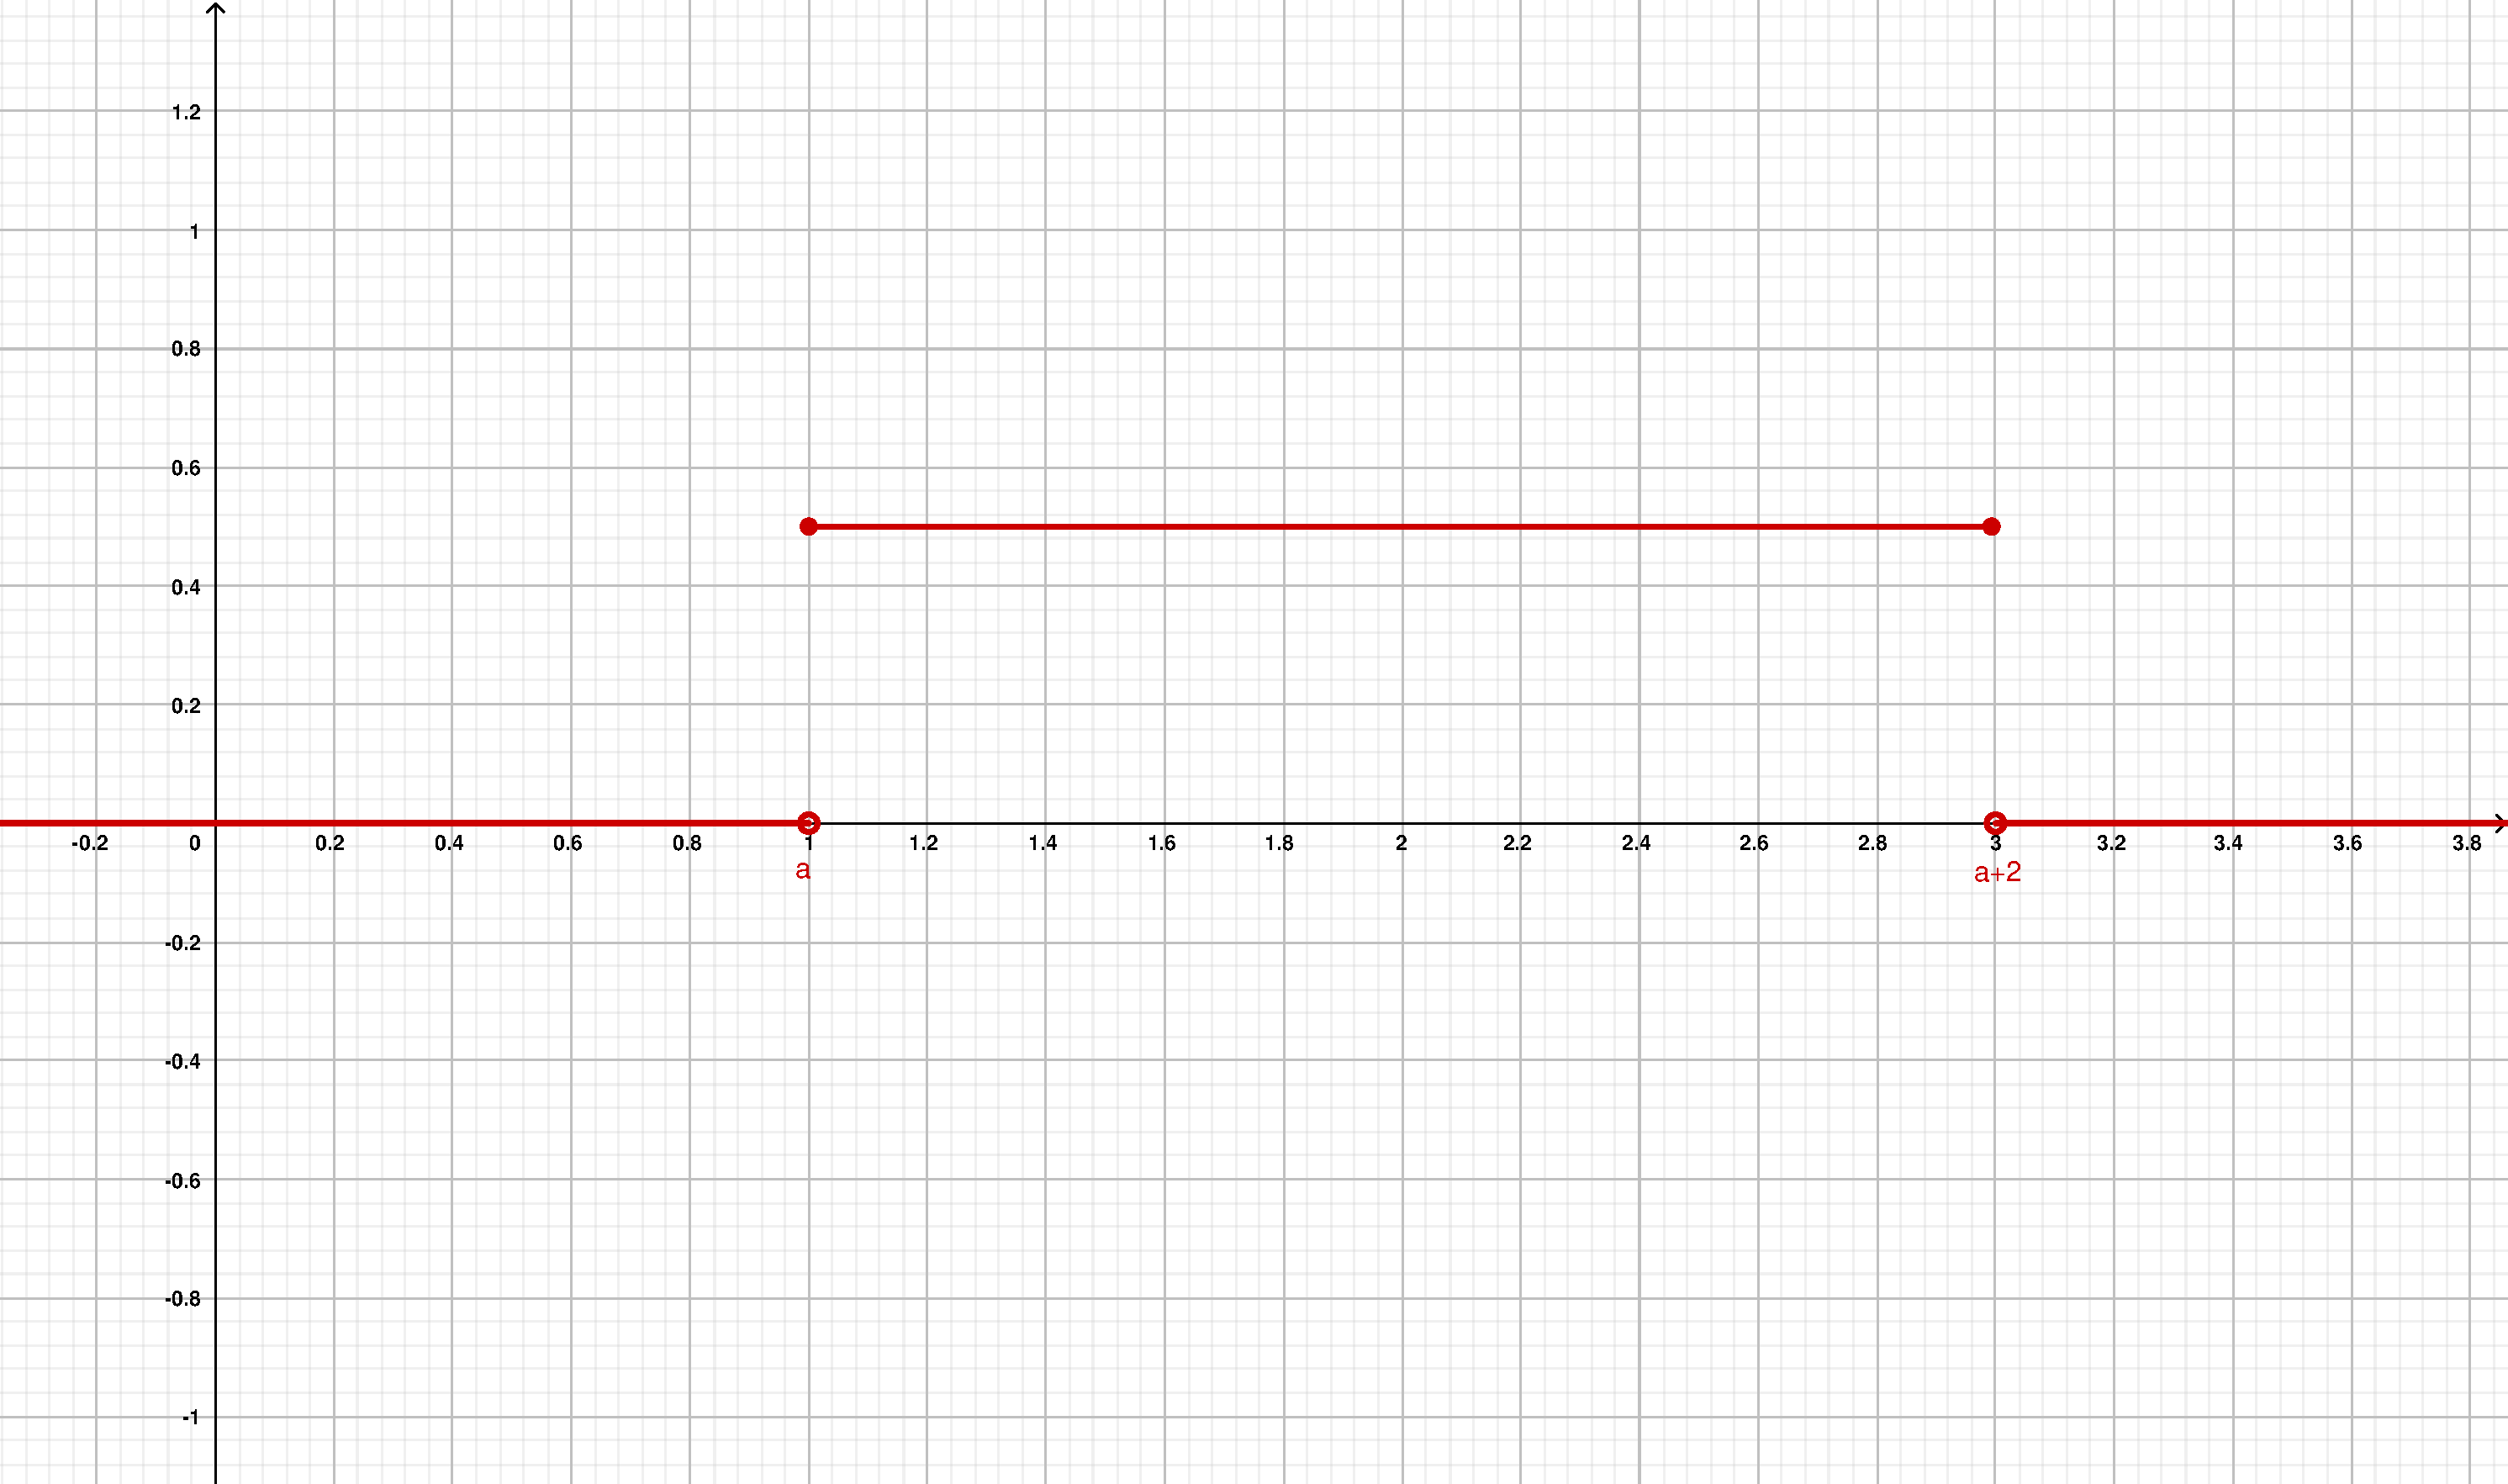
\includegraphics[width=0.6\linewidth]{pdf2}}
		\caption{The plot of probability density functions}
		\label{pdf}
	\end{figure}

	\textbf{Subproblem (b)}
	
	$\circ$ When $X=\frac{1}{2}$, we can have
	\begin{equation}
		\label{eq1}
		\begin{split}
			p\left(Y=0\mid X=\frac{1}{2}\right)&=\frac{p\left(Y=0\right)\cdot p\left(X=\frac{1}{2}\mid Y=0\right)}{p\left(X=\frac{1}{2}\right)}
			=\frac{\frac{1}{2}\cdot e^{-\frac{1}{2}}}{p\left(X=\frac{1}{2}\right)}\\
			p\left(Y=1\mid X=\frac{1}{2}\right)&=\frac{p\left(Y=1\right)\cdot p\left(X=\frac{1}{2}\mid Y=1\right)}{p\left(X=\frac{1}{2}\right)}
			=\frac{\frac{1}{2}\cdot p\left(X=\frac{1}{2}\mid Y=1\right)    }{p\left(X=\frac{1}{2}\right)}\\
			&\le\frac{\frac{1}{2}\cdot \frac{1}{2}}{p\left(X=\frac{1}{2}\right)}<\frac{\frac{1}{2}\cdot e^{-\frac{1}{2}}}{p\left(X=\frac{1}{2}\right)}=p\left(Y=0\mid X=\frac{1}{2}\right)
		\end{split}
	\end{equation}
	As we can see from equation \ref{eq1}, the conditional probability $p\left(Y=0\mid X=\frac{1}{2}\right)$ is larger than $p\left(Y=1\mid X=\frac{1}{2}\right)$. Thus, the most likely value of $Y$ is 0.
	
	$\circ$ When $X=1$, we can have
	\begin{equation}
		\label{eq2}
		\begin{split}
			p\left(Y=0\mid X=1\right)&=\frac{p\left(Y=0\right)\cdot p\left(X=1\mid Y=0\right)}{p\left(X=1\right)}
			=\frac{\frac{1}{2}\cdot e^{-1}}{p\left(X=1\right)}\\
			p\left(Y=1\mid X=1\right)&=\frac{p\left(Y=1\right)\cdot p\left(X=1\mid Y=1\right)}{p\left(X=1\right)}
			=\frac{\frac{1}{2}\cdot p\left(X=1\mid Y=1\right)}{p\left(X=1\right)}\\
		\end{split}
	\end{equation}
	According to equation \ref{eq2}, we can see that different value of $a$ will result in different conclusion.
	
	\begin{enumerate}[\qquad $\bullet$]
		\item $1\in[a, a+2]$

		In this situation, we have 
		\begin{equation}
			\label{eq3}
			\begin{cases}
				a \ge 0\\
				a \le 1\\
				a+2\ge 1\\
			\end{cases}
			\Longrightarrow
			a\in\left[0,1\right]
		\end{equation}
		Then, we can have
		\begin{equation}
			\label{eq4}
			\begin{split}
				p\left(Y=1\mid X=1\right)&=\frac{\frac{1}{2}\cdot p\left(X=1\mid Y=1\right)}{p\left(X=1\right)}=\frac{\frac{1}{2}\cdot \frac{1}{2}}{p\left(X=1\right)}\\
				&>\frac{\frac{1}{2}\cdot e^{-1}}{p\left(X=1\right)}=p\left(Y=0\mid X=1\right)
			\end{split}
		\end{equation}
		As we can see from equation \ref{eq3} and \ref{eq4}, when $a\in\left[0,1\right]$, the conditional probability $p\left(Y=0\mid X=1\right)$ is less than $p\left(Y=1\mid X=1\right)$. Thus, the most likely value of $Y$ is 1.
		\item $1\notin[a, a+2]$
		
		In this situation, we have 
		\begin{equation}
			\label{eq5}
			\begin{cases}
				a \ge 0\\
				a > 1 \,\, \text{or} \,\, a+2<1\\
			\end{cases}
			\Longrightarrow
			a\in\left(1,+\infty\right)
		\end{equation}
		Then, we can have
		\begin{equation}
			\label{eq6}
			\begin{split}
				p\left(Y=1\mid X=1\right)&=\frac{\frac{1}{2}\cdot p\left(X=1\mid Y=1\right)}{p\left(X=1\right)}=\frac{\frac{1}{2}\cdot 0}{p\left(X=1\right)}=0\\
				&<\frac{\frac{1}{2}\cdot e^{-1}}{p\left(X=1\right)}=p\left(Y=0\mid X=1\right)
			\end{split}
		\end{equation}
		As we can see from equation \ref{eq5} and \ref{eq6}, when $a\in\left(1,+\infty\right)$, the conditional probability $p\left(Y=0\mid X=1\right)$ is larger than $p\left(Y=1\mid X=1\right)$. Thus, the most likely value of $Y$ is 0.
	\end{enumerate}
	
	
\end{homeworkProblem}

\begin{homeworkProblem}
	[10 points] Markov's inequality is the most elementary tail bound which means that if a non-negative random variable $X$ has finite mean, then we have
	$$
	\operatorname{Pr}[X \geq t] \leq \frac{E[X]}{t} \quad \forall t>0
	$$
	For a random variable $X$ with finite variance, then show that it satifies the Chebyshev's inequality
	$$
	\operatorname{Pr}[|X-\mu|] \geq t] \leq \frac{\operatorname{Var}(X)}{t^{2}} \quad \forall t>0
	$$
	
	\vspace{4pt}
	\textbf{\large{Solution}}
	
	We set $D = \left\{x:|x-\mu|\ge t\right\}$, thus we have 
	\begin{equation}
		\label{eq7}
		\frac{|x-\mu|}{t}\ge 1,\quad x\in D
	\end{equation}
	Then, we set $f(x)$ as the probability density function of $X$, so we have
	\begin{equation}
		\begin{split}
			\text{Pr}\left[|X-\mu|\ge t\right] &= \int_{D}f(x)dx =\int_{D}1\cdot f(x)dx \\
			&\le \int_{D}\frac{|x-\mu|}{t}\cdot f(x)dx \quad(\text{euqation \ref{eq7}})\\
			&\le \int_{D}\left(\frac{|x-\mu|}{t}\right)^2\cdot f(x)dx\quad(\text{euqation \ref{eq7}})\\
			&=\frac{1}{t^2}\int_{D}\left(x-\mu\right)^2\cdot f(x)dx\\
			&\le \frac{1}{t^2}\int_{-\infty}^{+\infty}\left(x-\mu\right)^2\cdot f(x)dx\\
			&=\frac{E\left[\left(X-\mu\right)^2\right]}{t^2}=\frac{\text{Var}\left(X\right)}{t^2}
		\end{split}
	\end{equation}
		
\end{homeworkProblem}

\begin{homeworkProblem}
	[20 points] Let $X \in R^{m \times n}$ be a matrix of full column rank. Show that
	$$
	\min _{\theta \in R^{n}}\|y-X \theta\|_{2}^{2}=\left\|P_{b_{n}}^{\perp} \cdots P_{b_{2}}^{\perp} P_{b_{1}}^{\perp} y\right\|_{2}^{2},
	$$
	where $b_{1}=x_{1}, b_{2}=P_{b_{1}}^{\perp} x_{2}, b_{3}=P_{b_{2}}^{\perp} P_{b_{1}}^{\perp} x_{3}, \cdots, b_{n}=P_{b_{n}-1}^{\perp} \cdots P_{b_{2}}^{\perp} P_{b_{1}}^{\perp} x_{n} .\left(\right.$ Hint: $P_{b_{i}}^{\perp}$ is the projection of
	orthogonal complementary space of $\left.b_{i} .\right)$
	
	\vspace{4pt}
	\textbf{\large{Solution}}
	
	Because $X$ is a matrix of full column rank, we have that $\left\{x_i\right\}, i=1,2,\dots, n$ are linearly independent and the solution of $\operatorname{argmin} _{\theta \in R^{n}}\|y-X \theta\|_{2}^{2}$ is $\hat{\theta}=\left(X^{T} X\right)^{-1} X^{T} y$. Then we can have:
	\begin{equation}
		\min_{\theta \in R^{n}}\|y-X \theta\|_{2}^{2} = \|y-X\left(X^{T} X\right)^{-1} X^{T} y \|_{2}^{2} = \|\left(I-P\right)y\|_{2}^{2}
	\end{equation}
	where $P=X\left(X^{T} X\right)^{-1} X^{T}$ is the projection matrix onto the range space $\mathcal{R}\left(X\right)$, thus, $I-P$ is the projection matrix onto the orthogonal complement space of $\mathcal{R}\left(X\right)$.
	
	$\bullet$ Then, we would like to prove that $P_{b_k}^{\perp}b_k=0$. We know that the vector $b_k$ can be decomposed uniquely onto the space ${b_k}^{\perp}$ ans space $R^m-{b_k}^{\perp}+\left\{0\right\}$. So we have
	\begin{equation}
		\begin{split}
			b_k &= P_{b_k}^\perp b_k + P_{R^m-{b_k}^\perp+\left\{0\right\}} b_k\\
			&=P_{b_k}^\perp b_k+b_k\\
		\end{split}
		\Longrightarrow P_{b_k}^\perp b_k = 0
	\end{equation}
	Thus, we can have (suppose $i>j$)
	\begin{equation}
		\begin{split}
			b_i\cdot b_j &= \left\langle P_{b_{i-1}}^{\perp}\dots P_{b_2}^{\perp}P_{b_1}^{\perp}x_i, b_j\right\rangle\\
			&= \left\langle P_{b_{i-1}}^{\perp}\dots P_{b_{j-1}}^{\perp}P_{b_{j+1}}^{\perp}\dots P_{b_2}^{\perp}P_{b_1}^{\perp}x_i, P_{b_j}^{\perp}b_j\right\rangle\\
			&= \left\langle P_{b_{i-1}}^{\perp}\dots P_{b_{j-1}}^{\perp}P_{b_{j+1}}^{\perp}\dots P_{b_2}^{\perp}P_{b_1}^{\perp}x_i, 0\right\rangle\\
			&=0 \quad \left(\forall i\neq j\right)
		\end{split}
	\end{equation}
	since $P_{b_k}^{\perp}$ is self-adjoint and $P_{b_k}^{\perp}x_k=0$. Thus, $\left\{b_i\right\}, i=1,2,\dots, n$ are orthogonal to each other, so they are independent to each other. Then, we can have $W = \operatorname{span}\left\{b_1, b_2, \dots,b_n\right\} = \operatorname{span}\left\{x_1,x_2,\dots x_n\right\}=\mathcal{R}\left(X\right)$.
	
	$\bullet$ Then, we would like to prove that $P_{b_{n}}^{\perp} \cdots P_{b_{2}}^{\perp} P_{b_{1}}^{\perp}$ is the projection matrix onto the orthogonal complement space of $W$. Choose a vector $\boldsymbol{u}\in \mathbb{R}^m$, it is equal to prove that $\boldsymbol{v} = P_{b_{n}}^{\perp} \cdots P_{b_{2}}^{\perp} P_{b_{1}}^{\perp}\boldsymbol{u}\in W^\perp$. Then it is euqal to prove that $\boldsymbol{v}$ is orthogonal to any vector in $W$. We denote the vector $\boldsymbol{w_i}\in W$ as follow
	\begin{equation}
		\boldsymbol{w_i} = a_1b_1+a_2b_2+\dots+a_nb_n
	\end{equation}
	Thus, we have
	\begin{equation}
		\begin{split}
			\boldsymbol{v}\cdot \boldsymbol{w_i} &= \left\langle P_{b_{n}}^{\perp} \cdots P_{b_{2}}^{\perp} P_{b_{1}}^{\perp}\boldsymbol{u}, a_1b_1+a_2b_2+\dots+a_nb_n\right\rangle\\
			&=\left\langle P_{b_{n}}^{\perp} \cdots P_{b_{2}}^{\perp} P_{b_{1}}^{\perp}\boldsymbol{u}, a_1b_1\right\rangle + \left\langle P_{b_{n}}^{\perp} \cdots P_{b_{2}}^{\perp} P_{b_{1}}^{\perp}\boldsymbol{u}, a_2b_2\right\rangle+\dots+\left\langle P_{b_{n}}^{\perp} \cdots P_{b_{2}}^{\perp} P_{b_{1}}^{\perp}\boldsymbol{u}, a_nb_n\right\rangle\\
			&=\left\langle P_{b_{n}}^{\perp} \cdots P_{b_{3}}^{\perp}P_{b_{2}}^{\perp} \boldsymbol{u}, P_{b_{1}}^{\perp}a_1b_1\right\rangle + \left\langle P_{b_{n}}^{\perp} \cdots P_{b_{3}}^{\perp} P_{b_{1}}^{\perp}\boldsymbol{u}, P_{b_{2}}^{\perp}a_2b_2\right\rangle+\dots+\left\langle P_{b_{n-1}}^{\perp} \cdots P_{b_{2}}^{\perp} P_{b_{1}}^{\perp}\boldsymbol{u}, P_{b_{n}}^{\perp}a_nb_n\right\rangle\\
			&=0
		\end{split}
	\end{equation}
	Thus, $P_{b_{n}}^{\perp} \cdots P_{b_{2}}^{\perp} P_{b_{1}}^{\perp}$ is the projection matrix onto the orthogonal complement space of $W$, as well as the orthogonal complement space of $\mathcal{R}\left(X\right)$. Due to the unique of projection matrix, we have $P_{b_{n}}^{\perp} \cdots P_{b_{2}}^{\perp} P_{b_{1}}^{\perp}=I-P$, which shows that 
	\begin{equation}
	\min _{\theta \in R^{n}}\|y-X \theta\|_{2}^{2}= \|\left(I-P\right)y\|_{2}^{2}=\left\|P_{b_{n}}^{\perp} \cdots P_{b_{2}}^{\perp} P_{b_{1}}^{\perp} y\right\|_{2}^{2}
	\end{equation}
\end{homeworkProblem}

\begin{homeworkProblem}
	[50points] MLE for robust regression. Suppose we have the generative linear regression model
	$$
	Y=X \theta^{\star}+\varepsilon
	$$
	where $\varepsilon$ is the error term and $\varepsilon \sim N(0, \Sigma)$. The maximum likelihood estimator for $\theta$ is:
	$$
	\begin{aligned}
	\hat{\theta}_{L S} &=\operatorname{argmin}_{\theta \in R^{d}}\|X \theta-y\|_{2}^{2} \\
	&=\left(X^{T} X\right)^{-1} X^{T} y
	\end{aligned}
	$$
	
	\begin{itemize}
	    \item[(a)] Suppose the error term, $\varepsilon=\left[\varepsilon_{1}, \varepsilon_{2}, \cdots, \varepsilon_{n}\right]$ follows the Laplace distribution, i.e. $\varepsilon_{i} \stackrel{\text { i.i.d }}{\sim}$ $L(0, b), i=1,2, \cdots, n$ and the probability density function is $P\left(\varepsilon_{i}\right)=\frac{1}{2b} e^{-\frac{\left|\varepsilon_{i}-0\right|}{b}}$ for some $b>0$
	Under the MLE principle, what is the learning problem? Please write out the derivation process. (15 points)
	    \begin{figure}[!htbp]
	        \centering
	        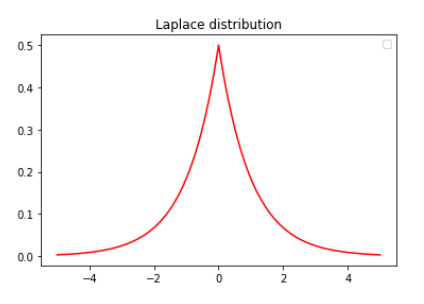
\includegraphics{tupian/laplacepdf.png}
	        \caption{PDF of Laplace distribution}
	        % \label{fig:my_label}
	    \end{figure}
	    
	    \item[(b)] \textbf{Huber-smoothing}. $L 1-$ norm minimization
	$$
	\hat{\theta}_{L 1}=\underset{\theta}{\operatorname{argmin}}\|X \theta-y\|_{1}
	$$
	is one possible solution for robust regression. However, it is nondifferentiable. We utilize smoothing technique for approximately solving the $L 1-$ norm minimization. Huber function is one possibility. The definition and sketch map are shown as below.
	$$
	h_{\mu}(z)\left\{\begin{array}{cl}
	|z|, & |z| \geq \mu \\
	\frac{z^{2}}{2 \mu}+\frac{\mu}{2}, & |z| \leq \mu
	\end{array}\right.
	$$
	\begin{figure}[!htbp]
	    \centering
	    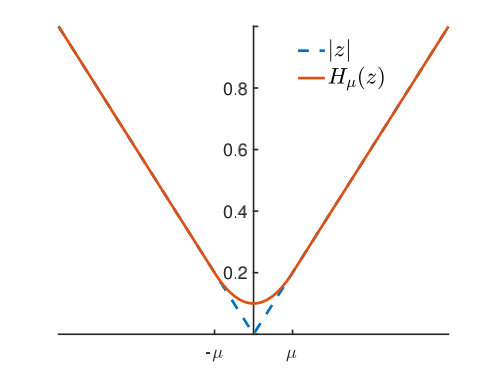
\includegraphics{tupian/Huber.png}
	    \caption{Huber smoothing}
	    % \label{fig:my_label}
	\end{figure}
	
	Then,
	$$
	H_{\mu}(Z)=\sum_{j=1}^{n} h_{\mu}\left(z_{j}\right)
	$$
	By using Huber smoothing, the approximation of the optimization of $L 1-$ norm can be changed to
	$$
	\min _{\theta} H_{\mu}(X \theta-y)
	$$
	Let
	$$
	f(\theta)=H_{\mu}(X \theta-y)
	$$
	find the gradient $\nabla f(\theta) .$ (10 points)
	   
	    \item[(c)] Gradient descent for minimizing $f(\theta)$. The process of gradient descent algorithm is shown in the following table.
	    
	\begin{algorithm2e}[h]
		\caption{\textbf{The Process of Gradient Descent Algorithm}}    
		\label{alg:GD}
		
		\lnlset{alg:fis-1}{1}{\textbf{Input}: observed data $X, y$ and initialization parameter $\theta_{0}$,
		\\Huber smoothing parameter $\mu$, 
		\\total iteration number $T$, 
		\\learning rate $\alpha$}.
		\\
		\lnlset{alg:pi-2}{2}\For{$k = 0,1,2, \cdots, T$}
		{
		\lnlset{alg:pi-3}{3}{$\quad \theta_{k+1}=\theta_{k}-\alpha \nabla f\left(\theta_{k}\right)$}
		}
		\lnlset{alg:pi-4}{4}{\textbf{end for}}
		
		\lnlset{alg:pi-5}{5}{\textbf{return} $\theta_{T}$}
		
	\end{algorithm2e}
	
	The data set is generated by the linear model
	$$
	Y=X \theta^{\star}+\varepsilon_{1}+\varepsilon_{2}
	$$
	
	where $\varepsilon_{1} \in R^{n}$ follows Gaussian distribution, $\varepsilon_{2}$ are outliers. Given the observed data $(x, y)=$ $\left\{\left(x_{1}, y_{1}\right),\left(x_{2}, y_{2}\right), \cdots,\left(x_{n}, y_{n}\right)\right\}$ and true value $\theta^{\star},$
	\begin{enumerate}[(1)]
	\item calculate the estimation $\hat{\theta}_{L S}$ by using linear least squares and compute $\left\|\hat{\theta}_{L S}-\theta^{\star}\right\|_{2} \cdot(5$ points)
	\item suppose $n=1000, d=50,$ use python to implement the gradient descent algorithm to minimize $f(\theta)$, the parameters are set as $\mu=10^{-5}, \alpha=0.001, T=1000,$ plot the error $\left\|\theta_{k}-\theta^{\star}\right\|_{2}$ as a function of iteraction number. You can download the data $\left\{Y, X, \theta^{\star}\right\}$ from Blackboard. (20 points)
	\end{enumerate}
	    
	\end{itemize}
		
	\vspace{4pt}
	\textbf{\large{Solution}}
	
	\vspace{4pt}
	\textbf{Subproblem (a)}
	
	Our model is 
	\begin{equation}
		y_i = \textbf{\textit{x}}_i^\top\boldsymbol{\theta}
	\end{equation}
	To be more explicit, consider
	\begin{equation}
		y_i = \textbf{\textit{x}}_i^\top\boldsymbol{\theta} + \epsilon_i \quad \text{with}\quad \epsilon_i\sim L(0, b)
	\end{equation}
	where $\epsilon_i$ are i.i.d. for $i = 1,\cdots,n$.
	
	Equivalently,
	\begin{equation}
		\epsilon_i = y_i - \textbf{\textit{x}}_i^\top\boldsymbol{\theta}\sim L(0, b)
	\end{equation}
	Thus, we can get the likelihood function as follow
	\begin{equation}
		\begin{split}
			L(\boldsymbol{\theta}) &= \prod_{i=1}^{n}P(\epsilon_i)=\prod_{i=1}^{n}\frac{1}{2b}e^{-\frac{\left|\epsilon_i\right|}{b}}\\
			&=(2b)^{-n}e^{-\frac{\sum_{i=1}^{n}\left|\epsilon_i\right|}{b}}
		\end{split}
	\end{equation}
	Then, we can get the $\log$-likelihood function as follow
	\begin{equation}
		\begin{split}
			\log L(\boldsymbol{\theta}) &= -n\log(2b)-\frac{1}{b}\sum_{i=1}^{n}\left|\epsilon_i\right|\\
			&=\text{Constant} - \frac{1}{b}\sum_{i=1}^{n}\left|\epsilon_i\right|
		\end{split}
	\end{equation}
	In order to make log-likelihood function to reach maximum value, we can derive the learning problem as follow
	\begin{equation}
		\begin{split}
			\widehat{\boldsymbol{\theta}}_{MLE}&=\underset{\boldsymbol{\theta}}{\operatorname{argmin}}\sum_{i=1}^{n}\left|\epsilon_i\right|\\
			&=\underset{\boldsymbol{\theta}}{\operatorname{argmin}}\sum_{i=1}^{n}\left|y_i-x_i^{\top}\boldsymbol{\theta}\right|\\
			&=\underset{\boldsymbol{\theta}}{\operatorname{argmin}}\|\boldsymbol{y}-\boldsymbol{X} \boldsymbol{\theta}\|_1
		\end{split}
	\end{equation} 
	
	\vspace{4pt}
	\textbf{Subproblem (b)}
	
	We can derive the gradient of $f\left(\boldsymbol{\theta}\right)$ as follow
	\begingroup
	\renewcommand*{\arraystretch}{1.5} 
		\begin{equation}
			\begin{split}
				\nabla f(\boldsymbol{\theta}) &=
				\begin{pmatrix}
					\frac{\partial f\left(\boldsymbol{\theta}\right)}{\partial\theta_1}\\
					\frac{\partial f\left(\boldsymbol{\theta}\right)}{\partial\theta_2}\\
					\vdots\\
					\frac{\partial f\left(\boldsymbol{\theta}\right)}{\partial\theta_d}
				\end{pmatrix}
				=
				\begin{pmatrix}
					\frac{\partial H_{\mu}\left(\boldsymbol{X}\boldsymbol{\theta}-\boldsymbol{y}\right)}{\partial\theta_1}\\
					\frac{\partial H_{\mu}\left(\boldsymbol{X}\boldsymbol{\theta}-\boldsymbol{y}\right)}{\partial\theta_2}\\
					\vdots\\
					\frac{\partial H_{\mu}\left(\boldsymbol{X}\boldsymbol{\theta}-\boldsymbol{y}\right)}{\partial\theta_d}
				\end{pmatrix}
				=
				\begin{pmatrix}
					\frac{\partial\sum_{i=1}^{n}h_u\left(\boldsymbol{x}_i^{\top}\boldsymbol{\theta}-y_i\right)}{\partial\theta_1}\\
					\frac{\partial\sum_{i=1}^{n}h_u\left(\boldsymbol{x}_i^{\top}\boldsymbol{\theta}-y_i\right)}{\partial\theta_2}\\
					\vdots\\
					\frac{\partial\sum_{i=1}^{n}h_u\left(\boldsymbol{x}_i^{\top}\boldsymbol{\theta}-y_i\right)}{\partial\theta_d}
				\end{pmatrix}\\
				&=
				\begin{pmatrix}
					\sum_{i=1}^{n}\frac{\boldsymbol{x}_i^{\top}\boldsymbol{\theta}-y_i}{\operatorname{max}\left\{\left|\boldsymbol{x}_i^{\top}\boldsymbol{\theta}-y_i\right|, \mu\right\}}x_{i1}\\
					\sum_{i=1}^{n}\frac{\boldsymbol{x}_i^{\top}\boldsymbol{\theta}-y_i}{\operatorname{max}\left\{\left|\boldsymbol{x}_i^{\top}\boldsymbol{\theta}-y_i\right|, \mu\right\}}x_{i2}\\
					\vdots\\
					\sum_{i=1}^{n}\frac{\boldsymbol{x}_i^{\top}\boldsymbol{\theta}-y_i}{\operatorname{max}\left\{\left|\boldsymbol{x}_i^{\top}\boldsymbol{\theta}-y_i\right|, \mu\right\}}x_{id}
				\end{pmatrix}\\
				&=\boldsymbol{X}^{\top}\cdot
				\begin{pmatrix}
					\frac{\boldsymbol{x}_1^{\top}\boldsymbol{\theta}-y_1}{\operatorname{max}\left\{\left|\boldsymbol{x}_1^{\top}\boldsymbol{\theta}-y_1\right|, \mu\right\}}\\
					\frac{\boldsymbol{x}_2^{\top}\boldsymbol{\theta}-y_2}{\operatorname{max}\left\{\left|\boldsymbol{x}_2^{\top}\boldsymbol{\theta}-y_2\right|, \mu\right\}}\\
					\vdots\\
					\frac{\boldsymbol{x}_n^{\top}\boldsymbol{\theta}-y_n}{\operatorname{max}\left\{\left|\boldsymbol{x}_n^{\top}\boldsymbol{\theta}-y_n\right|, \mu\right\}}
				\end{pmatrix}
			\end{split}
		\end{equation}
	\endgroup
		
	\vspace{4pt}
	\textbf{Subproblem (c)}
	\begin{enumerate}[(1)]
		\item Since $n > d$, we suppose $\boldsymbol{X}\in\mathbb{R}^{n\times d}$ has full column rank. Thus, we can derive that $\boldsymbol{X}^{\top}\boldsymbol{X}\in\mathbb{R}^{d\times d}$ is invertible. Then, we can calculate $\hat{\boldsymbol{\theta}}_{LS}$ as follow
		\begin{equation}
			\hat{\boldsymbol{\theta}}_{LS}=\left(\boldsymbol{X}^{\top}\boldsymbol{X}\right)^{-1}\boldsymbol{X}^{\top}\boldsymbol{y}
		\end{equation}
		
		By using Python, we can compute $\left\|\hat{\boldsymbol{\theta}}_{LS}-\boldsymbol{\theta}^{\star}\right\|_2$, the result is as follow
		\begin{equation}
			\left\|\hat{\boldsymbol{\theta}}_{LS}-\boldsymbol{\theta}^{\star}\right\|_2 = 144.695
		\end{equation}
		The Python code to solve this problem is showed as follow
\begin{python}
import pandas as pd
import  numpy as np
X = pd.read_csv("Sample data of X.csv", header=0, index_col=0)
y = pd.read_csv("Sample data of y.csv", header=None)
theta_star = pd.read_csv("data of theta_star.csv", header=None)


X = np.array(X)
y = np.array(y)
theta_star = np.array(theta_star)

theta_LS = np.dot(np.dot(np.linalg.inv(np.dot(X.T, X)), X.T), y)
error = np.linalg.norm(theta_star - theta_LS, ord = 2)
print(error)
\end{python}
		\item By using Python, we can plot the error $\left\|\theta_{k}-\theta^{\star}\right\|_{2}$ as a function of iteraction number as Figure \ref{fig_iter}
		\begin{figure}[H]
		    \centering
		    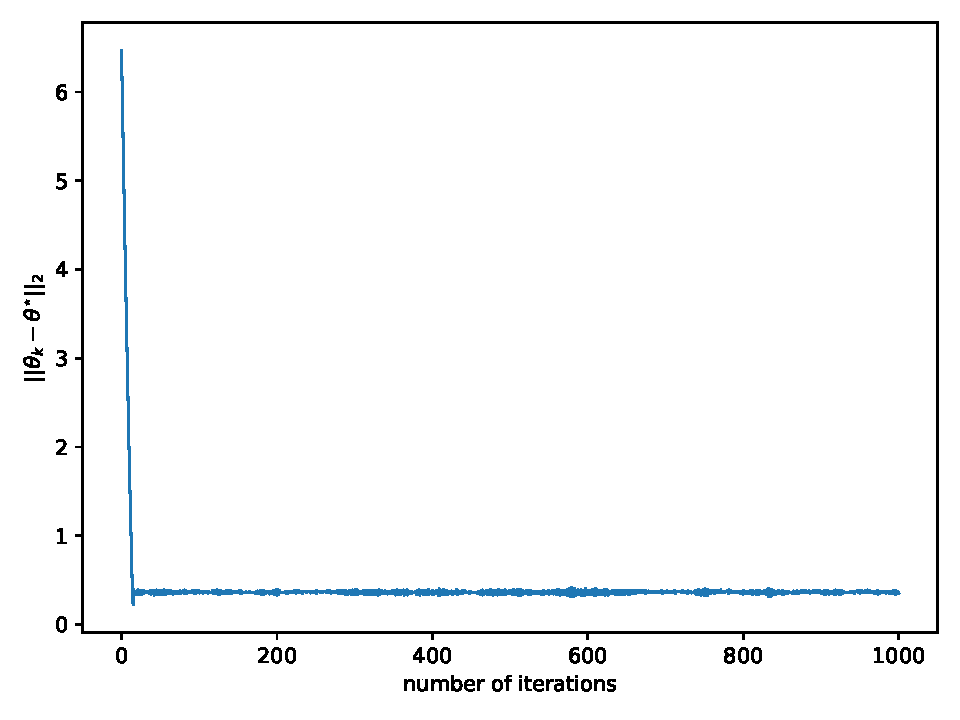
\includegraphics[width=0.6\linewidth]{tupian/plt.pdf}
		    \caption{Error $\left\|\boldsymbol{\theta}_{k}-\boldsymbol{\theta}^{\star}\right\|_{2}$ vs. iteraction number}
		    \label{fig_iter}
		\end{figure}
		The Python code to solve this problem is showed as follow
		\begin{python}
import pandas as pd
import numpy as np
import matplotlib.pyplot as plt

def hu(z):
    if abs(z) >= mu:
        return abs(z)
    else:
        return z*z/(2*mu) + mu/2
def f(theta):
    return sum(map(hu, np.dot(X, theta) - y))[0]

def df(theta):
    t = np.dot(X, theta) - y
    t1 = np.dot(X, theta) - y
    t[abs(t)>=mu] = abs(t)[abs(t)>=mu]
    t[abs(t)<=mu] = mu
    return np.dot(X.T, t1/t)

def GM(theta):
    thetak = theta
    norm_list = []
    norm_list.append(np.linalg.norm(thetak-theta_star))
    for k in np.arange(T):
        thetak = thetak - alpha * df(thetak)
        norm_list.append(np.linalg.norm(thetak-theta_star))
    norm_list = np.array(norm_list)  
    plot_convergence(norm_list)
    return thetak

def plot_convergence(norm_list):
    number = norm_list.size
    x = np.arange(number)
    #y = np.log(norm_list)
    y = norm_list
    plt.plot(x, y, linewidth=1)
    plt.xlabel('number of iterations')
    plt.ylabel(r'$||\theta_k-\theta^{\star}||_2$')
    plt.tight_layout()
    plt.savefig('./plt.pdf', dpi=1000)
      
X = pd.read_csv("Sample data of X.csv", header=0, index_col=0)
y = pd.read_csv("Sample data of y.csv", header=None)
theta_star = pd.read_csv("data of theta_star.csv", header=None)

X = np.array(X)
y = np.array(y)
theta_star = np.array(theta_star)

n = X.shape[0]
d = X.shape[1]
mu = 1e-5
alpha = 1e-3
T = 1000
theta0 = np.zeros(d).reshape(d,1)
thetaT = GM(theta0)
		\end{python}
	\end{enumerate}
	
	
\end{homeworkProblem}




\end{document}
